
%% bare_conf.tex
%% V1.4b
%% 2015/08/26
%% by Michael Shell
%% See:
%% http://www.michaelshell.org/
%% for current contact information.
%%
%% This is a skeleton file demonstrating the use of IEEEtran.cls
%% (requires IEEEtran.cls version 1.8b or later) with an IEEE
%% conference paper.
%%
%% Support sites:
%% http://www.michaelshell.org/tex/ieeetran/
%% http://www.ctan.org/pkg/ieeetran
%% and
%% http://www.ieee.org/

%%*************************************************************************
%% Legal Notice:
%% This code is offered as-is without any warranty either expressed or
%% implied; without even the implied warranty of MERCHANTABILITY or
%% FITNESS FOR A PARTICULAR PURPOSE!
%% User assumes all risk.
%% In no event shall the IEEE or any contributor to this code be liable for
%% any damages or losses, including, but not limited to, incidental,
%% consequential, or any other damages, resulting from the use or misuse
%% of any information contained here.
%%
%% All comments are the opinions of their respective authors and are not
%% necessarily endorsed by the IEEE.
%%
%% This work is distributed under the LaTeX Project Public License (LPPL)
%% ( http://www.latex-project.org/ ) version 1.3, and may be freely used,
%% distributed and modified. A copy of the LPPL, version 1.3, is included
%% in the base LaTeX documentation of all distributions of LaTeX released
%% 2003/12/01 or later.
%% Retain all contribution notices and credits.
%% ** Modified files should be clearly indicated as such, including  **
%% ** renaming them and changing author support contact information. **
%%*************************************************************************


% *** Authors should verify (and, if needed, correct) their LaTeX system  ***
% *** with the testflow diagnostic prior to trusting their LaTeX platform ***
% *** with production work. The IEEE's font choices and paper sizes can   ***
% *** trigger bugs that do not appear when using other class files.       ***
%                       ***
% The testflow support page is at:
% http://www.michaelshell.org/tex/testflow/



\documentclass[conference]{IEEEtran}


% *** CITATION PACKAGES ***
%
\usepackage{cite} % cite.sty was written by Donald Arseneau
% The latest version can be obtained at:
% http://www.ctan.org/pkg/cite
% The documentation is contained in the cite.sty file itself.


% *** GRAPHICS RELATED PACKAGES ***
%
\ifCLASSINFOpdf \usepackage[pdftex]{graphicx} \usepackage{wrapfig} % declare the
\graphicspath{{pic/}} % and their extensions so you won't have to specify these
\DeclareGraphicsExtensions{.png} \else % or other class option (dvipsone,
% dvipdf, if not using dvips). graphicx
% will default to the driver specified in the system graphics.cfg if no
% driver is specified.
% \usepackage[dvips]{graphicx}
% declare the path(s) where your graphic files are
% \graphicspath{{../eps/}}
% and their extensions so you won't have to specify these with
% every instance of \includegraphics
% \DeclareGraphicsExtensions{.eps}
\fi

% correct bad hyphenation here
% \hyphenation{op-tical net-works semi-conduc-tor}

\usepackage{textcomp} %\usepackage{svg}
%\setsvg{inkscape = inkscape -z -D, svgpath = svgs/}

\newcommand{\toolname}{Perquimans } \newcommand{\toolnameend}{Perquimans}
\newcommand{\toolnameposs}{Perquimans' }

\begin{document} \title{\toolnameend: A Tool for Visualizing Patterns of
		Spreadsheet Function Combinations}
	
	
	% author names and affiliations
	% use a multiple column layout for up to three different
	% affiliations
	\author{ \IEEEauthorblockN{Justin A. Middleton, Emerson Murphy-Hill}
		\IEEEauthorblockA{North Carolina State University, Raleigh, USA\\ \{jamiddl2,
			ermurph3\}@ncsu.edu }}
	
	% use for special paper notices
	%\IEEEspecialpapernotice{(Invited Paper)}
	
	% make the title area
	\maketitle
	
	% As a general rule, do not put math, special symbols or citations
	% in the abstract
	\begin{abstract} Spreadsheet environments often come equipped with an abundance
		of functions and operations to manipulate data, which users can combine into
		complex formulae. However, anticipating these
		combinations is difficult, complicating matters for both researchers and
		practitioners who want to study formulae to improve spreadsheet practices.
		Therefore, we developed \toolnameend, a tool that analyzes spreadsheet corpora
		to visualize patterns of function combination as an interactive tree, capable
		of representing both the most common and most anomalous patterns of formula
		construction and their contexts in actual workbooks. Using spreadsheets from
		the Enron corpus, we conduct both a case study and a user study to explore
		\toolnameposs various applications, particularly those in flexible smell
		detection and spreadsheet education.
		
	\end{abstract}
	
	\section{Introduction} Spreadsheets surround us. They serve key roles in
	industry, where as much as 95\% of U.S. financial firms use them
	daily~\cite{panko2008sarbanes}, and academia, where teachers can use them to
	track research and students' grades, not to mention many other
	applications~\cite{ko2011state}. It's this flexibility that grants them their
	allure: while a novice can still work without much experience, spreadsheets
	offer hundreds of specialized functions to fulfill a wide range of advanced
	needs, from complex statistics to text
	manipulation~\cite{nardi1990spreadsheet}. As such, it should be no surprise
	that tens of millions of workers rely on these programs
	daily~\cite{scaffidi2005estimating}.
	
	However, this ubiquity is not without danger; as more people adopt these tools
	and make larger and more complex sheets, the cost of failure grows too. To
	illustrate this, the European Spreadsheet Risks Interest Group (EuSpRIG)
	documents many horror stories of spreadsheets gone
	wrong\footnote{http://www.eusprig.org/horror-stories.htm}. One story tells of a
	2013 economics paper which drew connections between debt and national growth.
	Its findings shaped many political initiatives throughout the United States and
	Europe. However, other researchers soon discovered that a critical selection
	error in the research spreadsheets hampered the results and that, by correcting
	this error, the findings reversed completely! And this is only one of several
	accounts; even if most spreadsheet errors are relatively benign, poor
	spreadsheet practice can risk millions, if not billions, of
	dollars~\cite{powell2009impact}.
	
	From these stories, we can see the dire importance of understanding how people
	actually use spreadsheets. Fortunately, spreadsheet researchers have supported
	this by amassing spreadsheet collections from diverse sources, industrial to
	academic. Collections like EUSES~\cite{fisher2005euses},
	Fuse~\cite{barik2015fuse}, and the Enron corpus~\cite{hermans2015enron} have
	already fueled productive research across the field, such as in the search for
	code smells in spreadsheet environments~\cite{hermans2012detecting}~\cite{jansen2015code} or the creation of grammars to capture every possible
	spreadsheet program in Excel~\cite{aivaloglou2015grammar}. Additionally, some
	research has focused on comparing these collections, as Jansen did in 2015, to
	discover variation in spreadsheet techniques over time and
	location~\cite{jansen2015enron}.
	
	Considering the value of spreadsheets and all of these resources to describe
	their use, it becomes necessary that we design tools to better enable the
	exploration of these datasets and simplify the complex concepts that occur in
	spreadsheet design. One such concept is that of formula construction; functions
	are an important part of using spreadsheets efficiently, yet the number of
	potential combinations between them quickly becomes massive when you consider that
	there are hundreds of them. Tools, then, that empower people to explore
	questions about which functions are used together in practice have the
	potential to improve the current design of spreadsheets themselves and educate
	new generations of spreadsheets users on how to work best.
	
	This paper contributes such a tool, \toolnameend, that attempts to fulfill this
	need for better exploration by building on the aforementioned spreadsheet
	corpora. Working with spreadsheets in Excel, \toolname focuses primarily on the
	functions, like SUM and IF and hundreds more, which are the building blocks of
	formulae that determine values across a spreadsheet. The tool
	creates an interactive, exploratory visualization which captures how people
	combine these functions in a selected collection of spreadsheets, quantifying
	the broad patterns of function nesting while also being specific enough to find
	anomalous formulae and link them back to the specific cell in spreadsheets
	where they originate. \par
	
	Alongside the tool, we discuss several of the key decisions we faced during
	design, such as what to do with redundant formulae in a sheet or how to
	represent optional arguments, and we describe how our overall design goals both
	helped and hindered this process. We then apply the tool to a number of case
	studies to evaluate how much it could contribute to several different contexts,
	most notably code smell detection and spreadsheet education. To better understand how people might use \toolnameend, we also conducted a
	user study to judge how usable and intuitive the tool actually is. This grounds
	the discussion of its potential uses while also underscoring some of its
	inherent limitations and setting the way for future extensions and improvements
	upon the concept.
	
	\section{Related Work} \label{related-work} Visualizations excel for their
	ability to communicate information quickly and
	efficiently~\cite{baeza1999modern}; the visualization of spreadsheets,
	therefore, has offered much room for research. Several previous tools work
	within a spreadsheet, seeking to clarify the connections between the visible
	values in cells, the formulae that produce them, and the dependencies between
	cells that inform them. Igarashi and colleague's fluid
	visualizations~\cite{igarashi1998fluid}, for example, do this by imposing
	lines, color, and animation over the spreadsheet to visually explain these
	tangled connections. Likewise, Clermont explored ways of grouping cells by
	color and border that were related through similar functions, neighbors, or
	references~\cite{clermont2003scalable}, and Hipfl extended this work by
	incorporating the layouts and labels of spreadsheets~\cite{hipfl2008using}.
	Other tools focus on creating visualizations external to the sheets. Hermans
	and colleagues address a spreadsheet programmer's information needs by making
	dataflow diagrams from individual sheets through the tools
	GyroSAT~\cite{hermans2011supporting} and Breviz~\cite{hermans2011breviz}.
	\toolname is among the latter class, creating standalone visualizations about
	spreadsheets instead of drawing connections inside the spreadsheet itself. In
	contrast to the other visualization work, our work focuses on representing functions and how
	they combine into complex formulae, rather than exploring the data structures of any
	particular spreadsheet.  \par
	
	Many other tools inspect the structure of formulae but often from the
	perspective of finding bad design.  Following Fowler's initial description of
	code smells in object-oriented design~\cite{fowler2009refactoring}, many
	researchers have applied similar observations to spreadsheets and have
	cataloged classes of problematic
	formulae~\cite{hermans2012detecting}~\cite{cunha2012towards}~\cite{asavametha2012detecting}, often accompanying them with detection tools~\cite{abreu2014smelling} and investigations into real datasets~\cite{jansen2015code}. For example, Hermans, leveraging her work with the aforementioned dataflow diagrams, has worked with assessing common inter-worksheet smells, such as feature envy and inappropriate intimacy, wherein references between worksheets (rather than cells) in a file suggest a problem~\cite{hermans2012detectinginter}. Other tools, like Badame's Excel refactoring~\cite{badame2012refactoring}, are concerned more with understanding the formula in service of changing them. However, these studies define standards of poor design and orient their searches around them. Though \toolname supports the search for bad design, as we will see, the tool itself takes a much more agnostic approach in presentation, offering examples without regard for design quality. \par
	
	Implicit in this study is an exploration of the Excel API and how people use
	it. Previous research, such as the first study on the Enron
	spreadsheets~\cite{hermans2015enron} or in its comparison with the EUSUS
	corpus~\cite{jansen2015enron}, quantifies how often users employ certain
	functions but not how they combine them. Researchers have applied such
	questions to other contexts as well, such as Murphy and colleague's study into
	how Java developers use Eclipse and what commands they use most
	often~\cite{murphy2006java}. Others focus on the documentation of the API
	itself: Robillard and DeLine, for example conducted a series of surveys and
	interviews to diagnose common problems with learning APIs, and they found that
	code examples, one of the focuses of this tool, is one of the most important
	aids to have in learning a new system~\cite{robillard2011field}. Though this
	paper applies the tool to the Enron corpus specifically, the tool itself is not
	limited to this; it can be readily applied to any collection of Excel
	spreadsheets a user gives it.
	
	\section{Approach}
	
	\subsection{Design Goals} \label{goals} In visualizing the spreadsheet data, we
	set out a few core goals for what the tool should accomplish. Furthermore, with
	these goals, we also considered the likely challenges of achieving those goals
	and particular outcomes which we considered beyond the scope of the research.
	We present both sides of these goals below:
	
	\begin{itemize}
		
		\item [1] \textbf{Provide an interactive environment for free exploration.}
		There are a lot of data in some of these spreadsheet corpora, and the user
		should be able to pick for themselves which to explore while ignoring the
		rest. Furthermore, this exploration should not be designed around answering
		one specific question but rather helping to answer a variety of questions.
		
		\item [!1] \textbf{Do not make judgments about good and bad design.} Though
		users may certainly approach the tool with the intention of exploring
		particular formulae, a formula visualization tool will not prioritize any on
		metrics of good or bad practice.
		
		\item [2] \textbf{Emphasize the quantitative patterns in formula
			construction.} The tool should address the questions of how often the
		spreadsheet programmers used a certain function and where they used it. To do
		this, it must show metrics, such as frequency of use and depth of function
		nesting, of the dataset it conveys.
		
		\item [!2] \textbf{Do not overwhelm with numbers.} For popular functions
		especially, we anticipate that we'll have to show a lot of related data at
		once. Though everything should be accessible in accordance with Goal 1, we
		should design in a way that reduces noise.
		
		\item [3] \textbf{Promote a qualitative understanding of the patterns.} The
		tool should supplement its observations with concrete instances of relevant
		formulae from the corpus. Ideally, it should even direct users to the exact
		cell in the spreadsheets where the formula was used, contextualizing the
		functions.
		
		\item [!3] \textbf{Do not attempt to explain formulae.} Though the tool is meant
		to foster understanding by linking pattern to example, it will not try to be
		an explanatory tool that articulates what a complex formula accomplishes. Rather,
		we will provide the structure and context, and the user	must infer this on their own.
		
	\end{itemize}
	
	Though we kept these guidelines in mind through the development of \toolname,
	we nevertheless reached a number of points in which these principles
	conflicted. For a discussion of these decisions, see Section
	\ref{ssec:decisions}.
	
	\subsection{Walkthrough of the Tool} \label{sec:walkthrough}Before discussing
	the minutiae of tool's development, we will give a basic example of how to use
	the tool. For this, we will work from the visualization built on the Enron
	corpus to answer this question: \textit{ What kinds of functions do people use
		to define the condition in an IF function?} \par
	
	First, a word on the IF function. In Excel, it serves as one of the logical
	functions: given a condition as the first argument that evaluates to either
	true or false, it takes on the value of either the second or third argument,
	respectively. Or, as the documentation writes out, ``IF(Something is True, then
	do something, otherwise do something
	else)"\footnote{https://support.office.com/en-us/article/IF-function-69aed7c9-4e8a-4755-a9bc-aa8bbff73be2?ui=en-US\&rs=en-US\&ad=US}. Furthermore, the third argument is optional; if left out, the function will return a default ``FALSE" value if necessary. Examples of this function in practice can be seen in Figure~\ref{fig:ifexample}.
	
	\begin{figure}[h] \centering 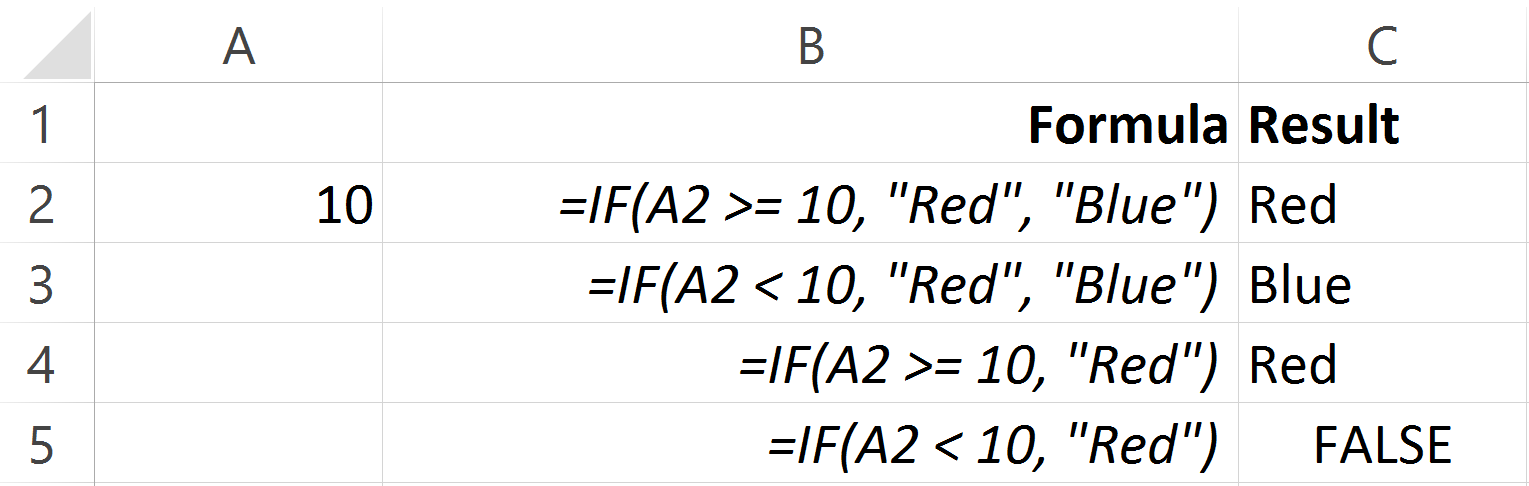
\includegraphics[scale=.9]{ifExample}
		\caption{Configurations of the IF function} \label{fig:ifexample} \end{figure}
	
	When the user first approaches the tree for a given top-level function -- that
	is, a function nested within none other -- only a few nodes are visible, as
	shown in Figure \ref{fig:startpic}. \par
	
	\begin{figure}[h] \centering 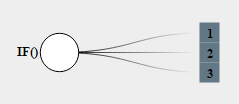
\includegraphics[scale=.4]{start} \caption{How the
			IF tree looks at the start} \label{fig:startpic} \end{figure}
	
	The visualization so far comprises two types of nodes: the circle
	
\includegraphics{glossary-greenonly}, which represents a discrete function in
	the formula and is size according to its frequency relative to the number of
	times the root function appeared; and the numbered squares
	
\includegraphics{glossary-blue}, which represent the positions of arguments
	within its parent function. From this, we can confirm that, of the times it was
	observed, IF can have at most three arguments passed into it, which corresponds
	with its specifications in the
	API. \par
	
	Knowing that it is the first argument which contains the conditionals, we click
	on the square labeled ``1" to explore. To save space, when the tool finds more than 10 unique
	arguments in a position, it displays only the first
	ten, with an option to display the rest by clicking the arrow
	
\includegraphics{glossary-arrow}.
	
	\begin{figure}[h] \centering 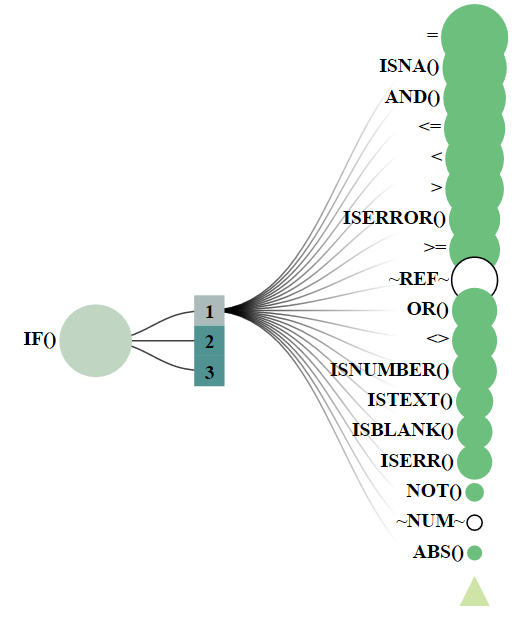
\includegraphics[scale=.4]{IFexpand}
		\caption{First argument of the IF tree} \label{fig:expandif} \end{figure}
	
	We see that IF contains a number of comparison operators as its first argument,
	such as = and $\le$, and boolean-returning functions, like ISNA and AND, with
	simple equality being the most common and ABS being the least. From here, we
	can further explore the common options among these functions. Clicking on the
	``=" node will yield two arguments and expanding each of them
	will peer into the range of common values of equality comparison, which Figure
	\ref{fig:fullpic} shows. \par
	
	\begin{figure*}[t] \centering 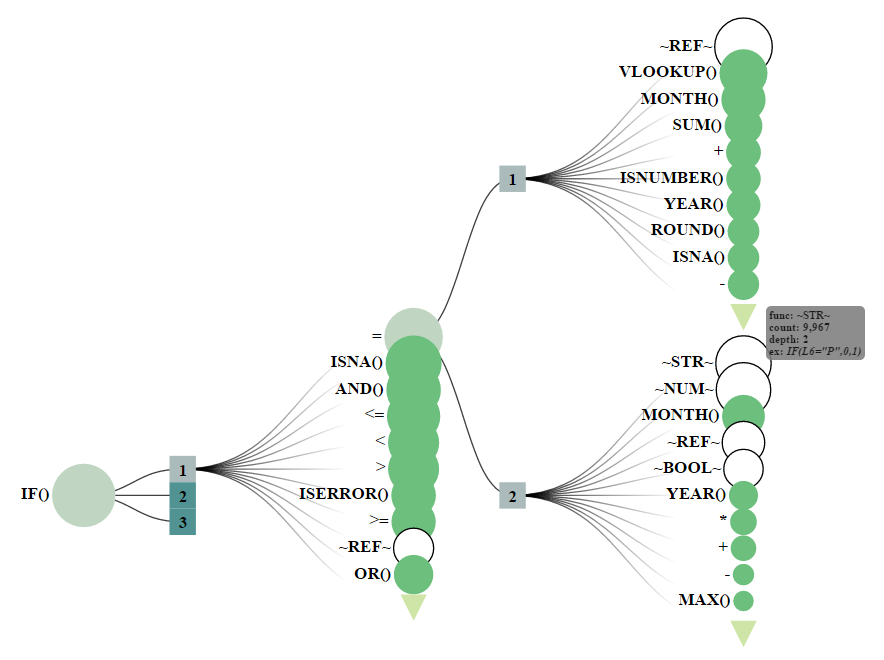
\includegraphics[scale=.5]{IFargslabel}
		\caption{A picture of \toolname displaying the common arguments to the IF
			function's first parameter} \centering \label{fig:fullpic} \end{figure*}
	
	For both sides of the equal sign, the operator has certain types of arguments
	which predominate over the others: on the left side is most often a reference
	to another cell; on the right, a string or number literal, which makes sense
	for the case of confirming a value in another cell before assigning this one.
	Furthermore, a tooltip accompanies each function node in the tree, providing a
	concrete example of a function that uses this structure. If this single
	instance is not enough, then the user also has the option to double-click the
	individual function node, which will open up a new tab with a table of many
	more examples from dataset.
	
	\subsection{Glyph Glossary}
	
	From these images, we can provide a quick glossary of glyphs within the
	visualization to aid interpretation. \begin{itemize} \item
		
\includegraphics{glossary-green} - \textbf{Function nodes} are green circles
		labeled with the function name. Their size is determined by their relative
		frequency, scaled logarithmically, to the frequency of the root node in the
		tree. They may have any number of arguments, including zero, as determined by
		the API. Users can select any of these nodes to view the examples from the 
		provided dataset that use this function in the node's position in the tree.
		
		\item \vspace{.25cm}
\includegraphics{glossary-leaf} - \textbf{Value nodes} are
		white circles with a generic label. They represent elements of a formula which
		accept no arguments, like references (A1), ranges (A1:A10), numbers, boolean
		values, strings, and errors. However, \toolname treats still functions with
		zero arguments, like NOW, as function nodes. Like function nodes, these also 
		contain examples.
		
		\item  \vspace{.25cm} 
\includegraphics{glossary-blue} - \textbf{Argument
			nodes} are dark blue squares labeled with a number. The number is the position
		of an argument within the function in the parent node. In Figure
		\ref{fig:expandif} for example, argument node 1 shows every function or value
		that was seen in the first argument.
		
		\item  \vspace{.25cm} 
\includegraphics{glossary-solidline} - \textbf{Solid
			lines} represent a function's list of parameters. As such, they
		connect the function nodes to argument nodes.
		
		\item  \vspace{.25cm} 
\includegraphics{glossary-fadingline} - \textbf{Fading
			lines} represents how a formula author can use several different possible
		functions or values within a single argument position. As such, they connect
		argument nodes to function or value nodes.
		
		\item  \vspace{.25cm} 
\includegraphics{glossary-arrow} - \textbf{Expansion
			arrows} appear within an argument node when there are over 10 possible
		functions or values in an argument position. By default, only the first 10
		will be shown along with this arrow; clicking this will show the rest as well.
		
		\item  \vspace{.25cm} 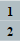
\includegraphics[scale=.75]{glossary-lightblue} -
		\textbf{Optional argument trees} are variations of trees that show only
		formulae with a specific number of arguments. For example, the function AND
		can take any number of arguments, up to 255. By default, the tree shows data
		from AND functions with any number of arguments, but these trees, which have argument nodes of a lighter blue color, can show how AND was used when \textit{only} two arguments
		were passed into it, or \textit{only} four, and so on. See
		Figure~\ref{fig:optional} for how the data between tree types differs.
	\end{itemize}
	
	\begin{figure}[h] \centering 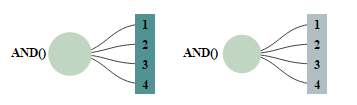
\includegraphics[width =
		.46\textwidth]{comparison} 
\includegraphics[]{comparison-ss} \caption{The
			contents of the default tree (left) and the optional argument trees (right)}
		\label{fig:optional} \end{figure}
	
	
	
	\subsection{Implementation Details} The visualization is the product of two
	discrete processes: \begin{itemize} \item \textit{Collection}: Given a set of
		Excel sheets, the tool, written in Java, uses Apache
		POI\footnote{https://poi.apache.org/} to identify and iterate over every cell
		containing a valid formula. Afterward, it calls POI's formula parser to break
		the formula text into an ordered set of individual tokens, which the tool then
		parses into the tree-like form. When all formulae have been analyzed like this,
		it produces JSON files for each top-level function in the set.
		
		\item \textit{Presentation}: The JSON files, meanwhile, feed into the
		presentation code, implemented in Javascript with much help from the
		visualization library D3\footnote{https://d3js.org/}. We chose D3 primarily
		for its accessibility: given the JSON, the visualization can be simply
		embedded into a webpage accessible through a browser. \end{itemize} A
	demonstration of \toolname can be found at
	https://github.com/DeveloperLiberationFront/Excel-Function-Visualizer.
	
	\subsection{Design Decisions} \label{ssec:decisions} Early in the design, we
	chose the tree form for its inherent ability to represent the parent-children
	relationship of formulae as functions and their arguments, which could be yet
	more functions. By adapting this structure for a broad range of
	possibilities for nested functions, the branching factor depends alternatively
	on the number of arguments in a function and the number of possible functions
	observed as an argument in a function. \par
	
	Another of our options was to represent the call trees as simple text hierarchies. 
	Though this might work well for a single, uncomplicated call structure, we did not
	do this because our tool combined many of these call trees into a more complicated 
	structure. To capture the different relationships in the tree and to quantify the
	frequency of arguments, we would need to be more verbose in our description. As such, we
	decided that visualizing some dimensions was quicker than writing them out. 
	\par
	
	Guided by the goals in Section \ref{goals}, we faced a number of decisions in
	how to visualize the data. Below, we've outlined those that
	had the largest impact in the values that appear in the tree. \begin{itemize}
		
		\item \textit{Copied formulae}: Excel allows users to spread a formula over an
		area, repeating the same task in each cell with minor adjustments. Without
		checking for this, the analysis may not reveal the functions most commonly
		used together but rather the formulae most often applied to large areas. To
		combat this, we converted formulae from their native A1 format to the relative
		R1C1, in which copied formulae should be identical, and considered only each
		R1C1 formulae once per worksheet.
		
		\item \textit{Importance of depth}: When a function appears within another,
		should it be analyzed only as a nested function or would it also be valid to
		analyze the nested function on its own? \par
		
		\ \ For example, in the pictured IF function, we found that people often use
		another IF statement as the second or third arguments of the top-level IF. If
		we only consider functions exactly where they're found embedded in the
		formula, then information about the same function -- IF, in this case -- will
		be scattered across different trees with no way to aggregate them. If we
		record every instance of a function by ignoring their context -- that is,
		including an IF embedded within a SUM function in the same node as the
		top-level IF -- then the tool will represent some functions in multiple nodes
		to capture every possible level of nesting. For now, we only include the
		first, with the latter to be added as an option in the future.
		
	\end{itemize}
	
	\section{Case Study} The obvious question to pose to any visualization is this:
	What do the images tell us that the text could not? It is not enough to prove
	that something can be visualized; we must also demonstrate what we can
	gain from any particular visualization. As such, we raised a few tasks in the
	introduction in which we thought the tool could help: detecting bad smells and
	guiding spreadsheet education. To demonstrate the tool's applicability, we
	sought out places in the tree which best exemplify these tasks.
	
	\subsection{Bad Smells} \label{badsmells} Fowler's description of code
	smells~\cite{fowler2009refactoring} underscored an important point of code
	quality: between elegant, efficient code and bug-crippled spaghetti, there is a
	spectrum of code designs which, by themselves, are not faulty but nevertheless
	suggest vulnerabilities in code design. Since then, researchers have applied
	these concepts to spreadsheet programming, as discussed in
	Section~\ref{related-work}. While some of the smells lie beyond the scope of
	the tool, such as those characterizing inter-worksheet connections, others have
	structures which create distinctive features within the tree, leading to easy
	detection through our visualization: \par
	
	\begin{itemize}
		
		\item \textit{Multiple Operations}: A single formula comprises numerous
		functions and operators~\cite{hermans2012detecting}. As a result, the formula
		tends to be prohibitively complex. In the visualization, since each nested and
		combined function creates yet another level of depth within the tree, these
		constructions can result in long, horizontal chains of nodes, as seen in
		Figure~\ref{fig:longsum}.
		
		\item \textit{Long Parameter List}: A function uses numerous arguments, making
		it harder to understand~\cite{asavametha2012detecting}. This is not a problem
		for many functions which have a limited number of arguments that it accepts.
		However, for functions that accept arguments indefinitely, such as SUM and
		CONCATENATE, it creates tall towers of argument nodes from a single function
		node.
		
		\item \textit{Conditional Complexity}: A logical function, particularly IF,
		nests several other logical functions inside of it, reducing code
		readability~\cite{hermans2012detecting}. These can be traced manually in the
		trees for the logical functions. IF, for example, will have several more IF
		function nodes within its second or third arguments, which in turn might have
		more of the same nested within them.
		
	\end{itemize}
	
	\begin{figure*}[h] \centering 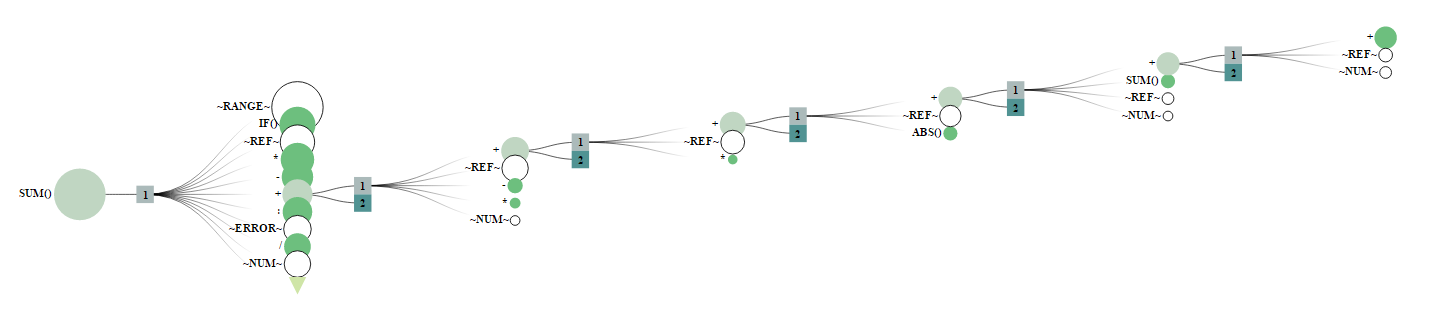
\includegraphics[width=\textwidth]{longsum}
		\caption{The horizontal length of a tree may indicate complex or redundant
			design} \label{fig:longsum} \end{figure*}
	
	Some code issues are meaningful not for the space they occupy but for how they
	clash with a function's expectations. For example, Excel offers a number of
	functions that accept any number arguments given to them, up to a
	resource-defined limit. SUM, for example, simply adds every argument given to
	it. This also means that it can accept only one argument, and when the user
	does so, they pass in a range of cells over 90\% of the time. However, using
	the tool, we isolated an instance where the programmer used a single-argument
	SUM where the argument was a series of 32 contiguous cells added with the +
	operation -- ``SUM(C6+C7+C8+C9+C10+C11+C12+C13+...+C37)" -- representing a
	technically valid but unusual and problematic design.\par
	
	However, because \toolname makes no judgments beforehand about which designs to
	emphasize as good or bad, the tool can be used to find strange or suboptimal
	designs that exist outside these readily visible categories. Consider the second
	argument of the ``='' operator, already shown expanded in
	Figure~\ref{fig:fullpic}: among the top five argument types for the position in
	an IF function were boolean values. This corresponds to designs in which
	conditions already in a boolean form were then checked against ``=TRUE" or
	``=FALSE", such as in the formula \textit{IF(Formulas!C77=TRUE, ``Yes")}, which
	appears in one of the sheets. Though this practice does not break anything in
	itself, it nevertheless represents redundant operations in formula design and
	indicates a possible misunderstanding of how the IF function works over the
	hundreds of examples of this boolean comparison that our tool can return.
	
	\subsection{Education} When Robillard and Deline researched common obstacles
	for programmers learning new APIs, they concluded that one of the most
	important elements of a good API was the use of code examples to demonstrate
	function use~\cite{robillard2011field}. Examples in APIs, furthermore, come in a variety of forms: small
	snippets or tutorials that show only the intended function, sample applications
	that incorporate the function in a broader context, or even production code
	that employs the function but was not initially intended to be an illustrative
	example. Of these categories, \toolname aligns
	entirely with the last; when a user chooses to explore a particular function
	node, they will see examples of that formula as it was used in a working
	environment, with the specifics depending on the dataset the tool is using.
	\par
	
	Furthermore, Robillard and Deline's study makes the case for examples that show
	``API usage patterns involving more than one method call"~\cite{robillard2011field}. Examples that show only a single function, they
	find, are too simple, whereas those demonstrating the interaction of functions
	will equip users for more complex tasks. \toolname is especially suited for
	this focus on combination; consider again the question in the walkthrough
	(Section \ref{sec:walkthrough}), asking which functions and operations are used
	as conditions in IF. The design of this tool emphasizes the connection, then,
	between what functions like ISNA and AND return and what IF accepts, and
	specific examples for any of these combinations are only a click away.
	
	%Lookup example
	For a deeper example, the LOOKUP functions are some of the most popular in
	Excel yet come with a number of important but silent requirements for proper
	use, and, as such, they have warranted some extra attention with regards to
	spreadsheet design. In short, these functions are for ``when you need to look in
	a single row or column and find a value from the same position in a second row
	or column"\footnote{https://support.office.com/en-us/article/LOOKUP-function-446d94af-663b-451d-8251-369d5e3864cb}. Examples of their use can be found in Figure \ref{fig:lookupexample}, and we will cover each type
	in more depth to better understand the visualizations for these functions.
	
	\begin{figure}[h] \centering 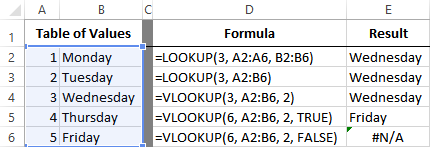
\includegraphics[width=.5\textwidth]{lookupexample}
		\caption{Demonstrations of LOOKUP and VLOOKUP} \label{fig:lookupexample}
	\end{figure}
	
	LOOKUP has two forms: vector and array. In either case, the first argument is
	the value which you are trying to match in another column. If the formula is in
	the vector form, that column is the second argument, so in Figure~\ref{fig:lookupexample}, 
	the formula in cell D2 (\textit{=LOOKUP(3, A2:A6,
		B2:B6)}) will search for the value of 3 between cells A2 and A6. The value the
	formula returns then comes from the corresponding cell in the optional third
	argument's column; since the lookup values matches the value in cell A4, it
	returns the value from cell B4. The array form of the LOOKUP works the same
	way, except that the second argument is a two-dimensional table where it
	matches values in the table's first column and returns values from the last.
	Also, depending on the dimensions of the lookup table, the function may
	substitute rows for columns.
	
	VLOOKUP works closely with this array form, except the user defines in its
	third argument which column from which to return values. In \textit{=VLOOKUP(3,
		A2:B6, 2)}, the argument ``2" tells to return the value from the second column,
	which is \textit{B2:B6} here. Furthermore, it also accepts a boolean value for
	an optional argument: when set to FALSE, it returns only exact matches, and
	when TRUE or left out, it approximates the match to the closest value beneath
	it. We demonstrate this in Figure~\ref{fig:lookupexample} in the bottom two
	VLOOKUP functions, one returning ``Friday" and the other an error. HLOOKUP
	works identically but focuses on rows instead of columns.
	
	All of these variations may seem daunting to a beginner, but \toolname can
	help. Because of its design, users can distinguish between forms of the same
	function, as seen in Figure~\ref{fig:lookups} where one can explore both
	the frequency with which the spreadsheet programmers used these different forms
	-- three-argument vector form much more than the array form -- and then
	retrieve examples of every configuration in the dataset. The same goes for the
	V/HLOOKUP functions, as shown partially in Figure~\ref{fig:vhlookups}.
	
	\begin{figure}[h] \centering 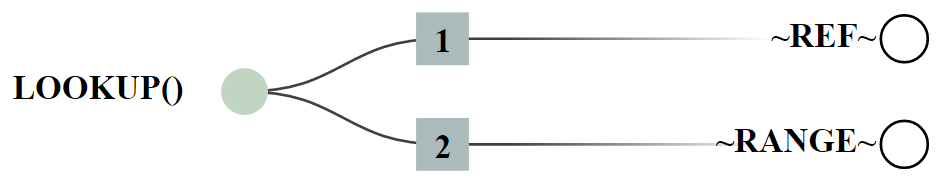
\includegraphics[width=.5\textwidth]{lookup-2}
		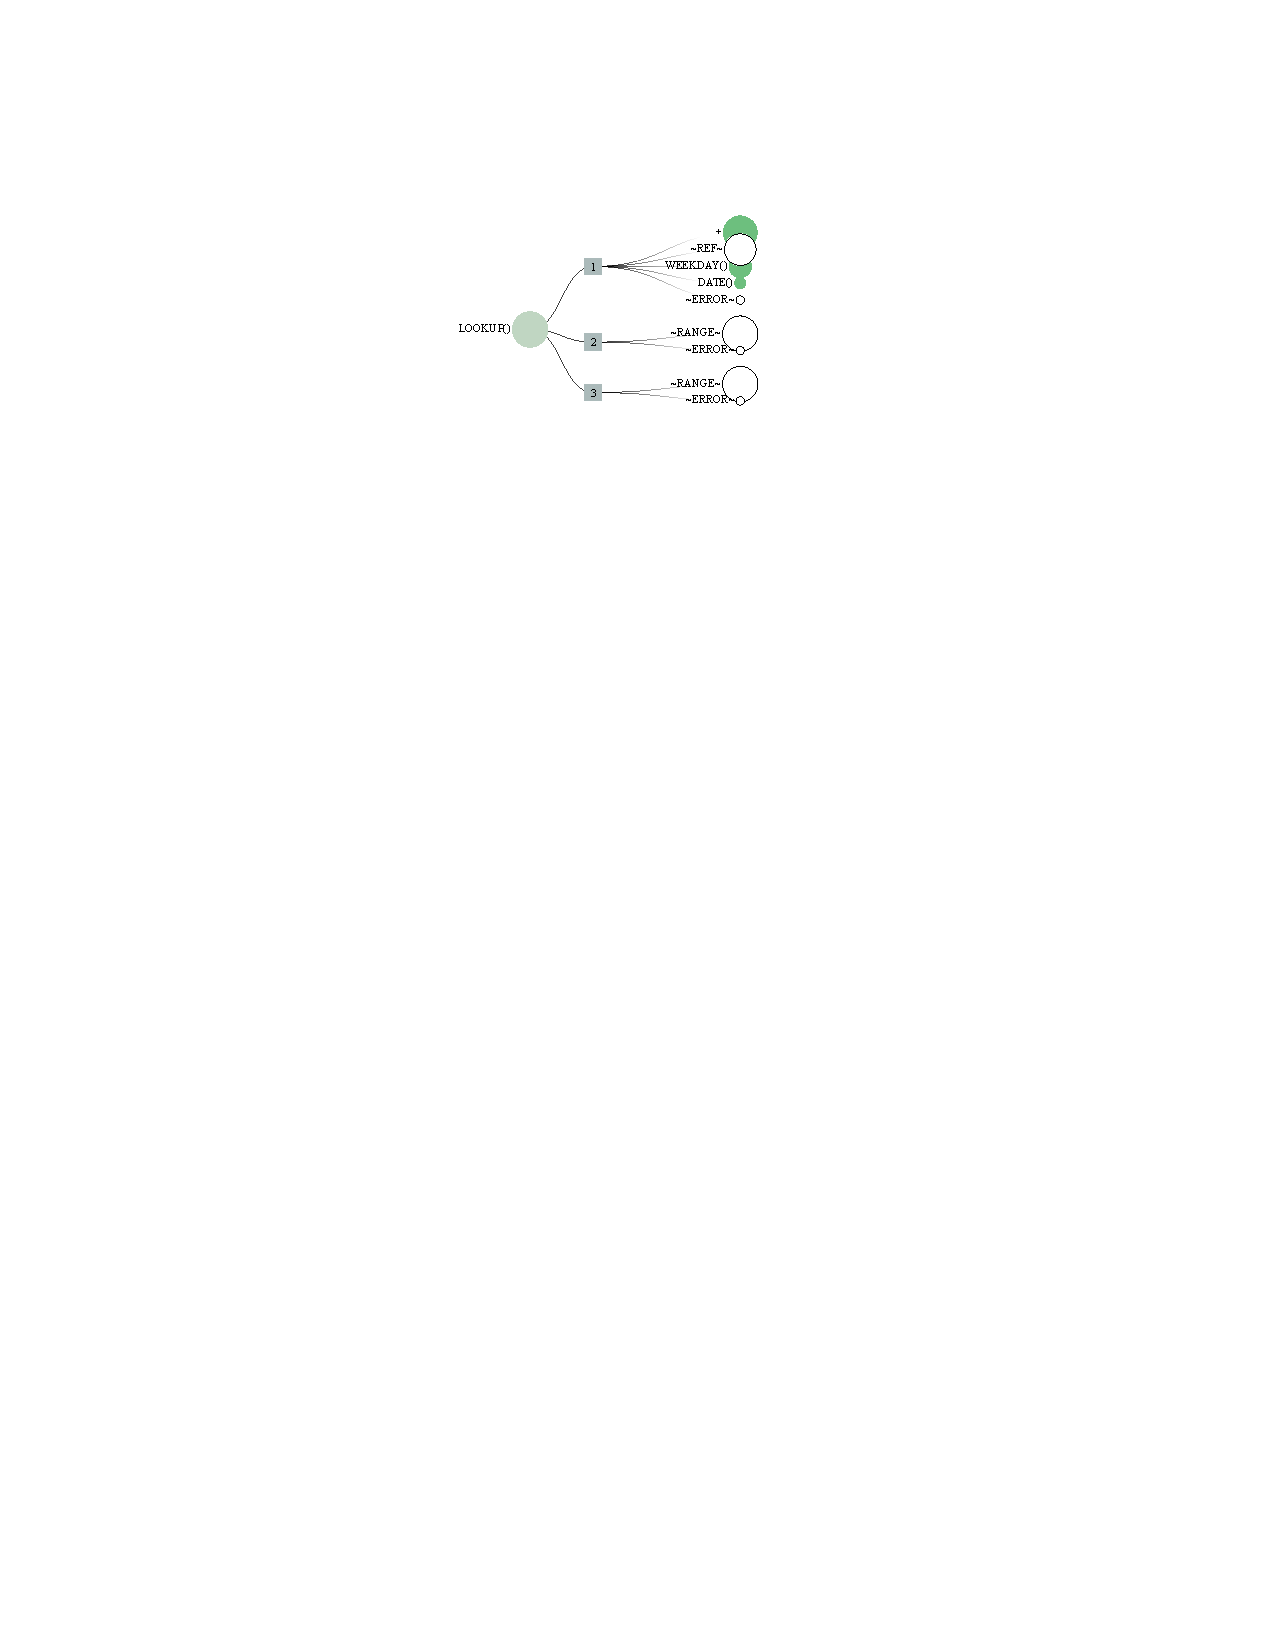
\includegraphics[width=.5\textwidth]{lookup-3} \caption{LOOKUP with two and
			three arguments}  \label{fig:lookups} \end{figure}
	
	Furthermore, these examples are good as well for exploring how it might bridge
	issues of bad design with education. In a recent study, Hermans and colleagues
	probed the Enron dataset for uses of VLOOKUP and HLOOKUP
	specifically~\cite{hermans2015detecting}. The issue at hand was the optional
	fourth argument, which requires that rows are sorted lest it return inaccurate
	results. For someone seeking to increase awareness of this problem, it first
	allows them to answer the question of significance -- ``How often do
	spreadsheet programmers use this function, with these particular
	parameters?" Though \toolname does not discern whether neighboring columns are
	sorted, it can nevertheless guide the educator to several examples in
	production where this problem surfaces. \par
	
	\begin{figure}[h] \centering 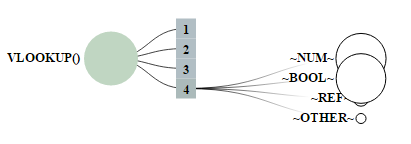
\includegraphics[width=.5\textwidth]{vlookup}
		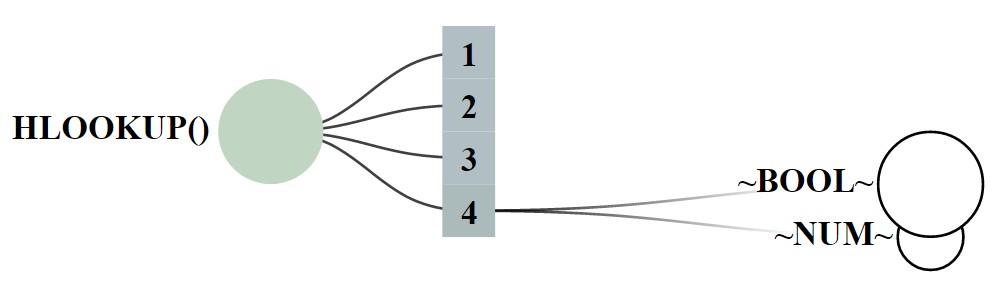
\includegraphics[width=.5\textwidth]{hlookup} \caption{VLOOKUP and HLOOKUP with
			four arguments} \label{fig:vhlookups}\end{figure}
	
	\section{User Study} \label{sec:userstudy} During development, we conducted a
	brief, four-participant user study to detect conflicts between our
	design and the goals in Section \ref{goals}. We designed the study to be
	exploratory; given trees based in the Enron dataset and at least twenty
	minutes, we asked the participants to adopt the persona of a consultant
	evaluating a company's spreadsheet practice, allowing for questions like which
	functions on which the employees most depended or which sheets or employees
	presented the most anomalous or dangerous designs. Though we instructed them on
	how to use the tool and suggested that they visit one of the most populous
	trees in the set, we put aside any specific tasks or questions and let them
	choose their own paths. Though interpretation of the phrase ``spreadsheet
	practice" can certainly vary from participant to participant, we readily
	accepted this interpretive flexibility since we wanted a range of views and
	backgrounds despite the persona. We clarified, furthermore, that their
	observations could be directed either at the quality of the data conveyed by
	the tool or at the tool's design itself. We present an overview of responses below, with the four participants
	recorded simply as P1 through P4. \par
	
	\subsection{Use in Smell Tracking} 
	
	The participants were most vocal about their findings when they discovered, by
	purpose or accident, instances of heinous design in the dataset. Many times,
	they noted these examples shortly after opening a new tree, suggesting that the
	distinctive visual signatures as discussed in Section \ref{badsmells} was a
	salient force in their exploration. For example, when P3 encountered the
	initial design of the SUM tree, as seen in Figure \ref{fig:sum}, they readily
	diagnosed that either a spreadsheet author was ``totally incompetent, or [the
	formula was] just something that's weird." Even though the visualization struggles
	to scale well for this formula, it calls clearly to a problem in the underlying
	spreadsheets -- awkward formulae make awkward trees. Other than these visual cues, value
	errors, prefixed with \#s, also appear in the tree, which P4 said could be
	useful for tracking these problems if marked well. 
	
	\begin{wrapfigure}{L}{.25\textwidth}
		\centering 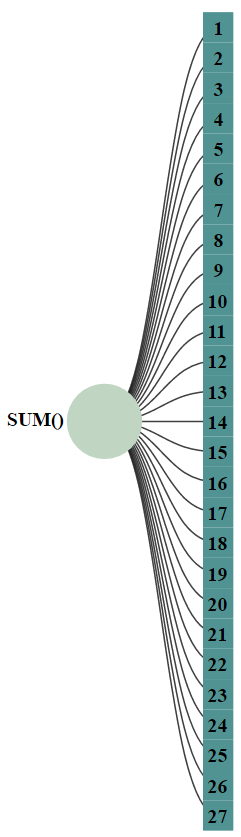
\includegraphics[width=.20\textwidth]{SUM}  \caption{An abundance of parameters in SUM, which was a commonly noted smell in the user study} \label{fig:sum} \end{wrapfigure}
	
	Additionally, because the Enron files had names with the author as a
	prefix, P2 commented that companies could use the tool to
	follow up with repeat offenders. For instance, they first encountered a
	particular author's name when investigating an AVERAGE function with 18
	distinct arguments for which our participant could not discern any logical
	order even after opening the source spreadsheet; the same name popped up again
	as P2 looked at a RATE function relying on several hard-coded values. P2 said
	that, if they were a manager or project leader, this recurrence was a sign to
	talk to the author personally and figure out why these problems were there, as
	to prevent more in the future. They also added that these problems would grow
	worse if this particular author left the company and no one remained who
	understood these formulae, a concern that aligns with Hermans' transfer
	scenarios \cite{hermans2011supporting}.
	
	The detection of bad design, however, is certainly not limited to a
	visualization tool. Some users remarked that a tool which printed a list of
	errors could work just as well for that purpose, and smell checkers can and
	have been directly built into spreadsheets to point out bad design.
	However, users also said that this visual interface is better when searching
	for new smells. Because the exploratory design makes no qualitative judgment
	and visualizes benign designs with the problematic, it allows for flexible
	interpretation of what a smell is; that is, a user might not realize a certain
	design is poor until they see it in the tree and, at the point, find specific
	examples of where it occurs in the spreadsheets.
	
	\subsection{Use in Education} Users found \toolname's inclusion of examples to
	be especially useful since none of the them considered themselves to be experts
	of Excel, their self-reported proficiencies ranging from ``fairly familiar" (P2)
	to ``not extremely familiar" (P4). For example, as P1 explored the VLOOKUP
	function, they said they could use the tool to collect more examples than the
	documentation offers even though they knew the documentation more verbosely
	explained its function signature. Furthermore, in the process of exploring
	trees, P1 and P3 also gravitated towards some functions they had not used
	before, such as PV and IPMT, looking for new features in Excel to explore and
	learn. \par
	
	Additionally, \toolname offers a simple way of finding examples where certain
	functions were used together, demonstrated when P4 took special interest in how people
	frequently used MATCH as the second argument of INDEX or how they used date functions
	like DATE and MONTH as lookup values in VLOOKUP. Though a standard text-search tool might yield
	the same results for a function alone, combinations can require more complex
	text queries, whereas here, the information is already captured in nodes.  \par
	
	However, we found that even though a user can explore all of a function's
	configurations, this does not mean that they will learn exactly what it does.
	P1, examining unfamiliar functions like KURT and PV, could describe precisely
	what types of arguments it accepted and how many. But even after exploring the
	spreadsheets for context, they could not accurately describe what the functions
	produced without consulting the official documentation. Whether through
	reticence of the tool or obscurity of the functions themselves, the exploratory
	environment is not enough to teach users \textit{when} to use a function.
	However, we could address this in future designs, perhaps, by linking directly
	to such documentation from within the tool without violating any design
	concerns in Section~\ref{goals}. \par
	
	\subsection{Study Limitations} Though we did not start the study by telling
	that the data source came from Enron, two users studied the file names to
	deduce its roots in finance, if not Enron itself. Because of these notorious
	connotations, then, they might have been inclined from this information to
	orient their exploration around finance-related functions, potentially limiting
	their findings or perceived users for the tool. However, one participant also said that,
	without this essential context, they could not have intelligently explored a dataset
	in the first place. Comments like these point out the trade-offs of unguided
	exploration, too: though it might not restrict them to a single purpose, it
	might, at the same time, not afford them any mindset at all with which to
	interpret the data. \par
	
	Furthermore, the data which users explored was processed and created before we
	had fully ensured that the tool could extract all of the useful data from the 
	spreadsheets, meaning some of the counts and patterns in the
	trees were inaccurate. However, we decided that this was not a pressing
	concern, being that we were primarily concerned with whether any interesting
	reports could be made at all, not with whether these reports were 100\%
	accurate assessments of reality. \par
	
	Throughout the study, we noticed that users misunderstood some of the icons
	and, as such, their early discoveries were inaccurate. For example, P1
	interpreted the numbers on the argument boxes to mean that all of the box's
	children had exactly that many arguments -- that is, clicking on the dark blue
	``1" would return all the single-argument functions instead of the first
	argument of a function -- and P2 initially took the solid lines to mean
	different paths in formula construction rather than different arguments of the
	same function. Though the users naturally did not explicitly report
	misinterpreting the icons, these misunderstandings became clear in their early
	evaluations of the spreadsheet practice. Though we clarified the meanings when
	these misunderstandings became apparent, these events point to a failure in the
	tool to indicate every function clearly.   \par
	
	
	\section{Limitations} We began these studies with the intention of evaluating
	our progress towards the goals in Section \ref{goals}. Working from these
	results, we noted many places where the tool aligned well or fell short.
	
	\subsection{Unbiased Exploration} The first goal -- that of full exploration --
	is threatened by the presence of certain formulae that the tool does not
	display, such as those with nonstandard functions. Because the data collection
	depends on POI's formula parser, it does not allow for any partial parsing of a
	formula; it either processes a formula perfectly or throws it out. As such, the
	visualization does not display anything with syntactical errors or third-party
	functions that POI cannot parse. This poses larger problems, however, when POI
	does not support the parsing of certain functions, such as EOMONTH, preventing
	the healthy growth of those trees. \par
	
	Other than that, we did avoid designing anything that intentionally evaluated
	formula designs. Nevertheless, \toolname inadvertently emphasizes bad design of
	certain types, such as all of those in Section~\ref{badsmells} marked by their
	visual signatures. Even so, our participants found the discovery of bad smell
	to be the most interesting aspect about it, to the point where they could
	imagine business scenarios in which micromanagers use it to ensure precise
	design parameters across a department's spreadsheets! To design in that
	direction, however, would mean a reevaluation of this design goal, since
	intentionally guiding users toward known smells may guide them away from new,
	unmarked ones.
	
	\subsection{Uncluttered Quantification}
	
	We realized early that some of the popular functions would have thousands of variations in large datasets, and showing all of
	these variations at once would hopelessly overwhelm the user. We therefore made
	a number of choices, such as the expansion arrows and the use of generic types
	in place of specific primitive values, that would reduce the variation to
	something more manageable.
	
	Nevertheless, during the user study, P3 remarked that they specifically avoided
	the most popular functions, anticipating a flood of nodes from which they could
	salvage nothing interesting. P2 corroborated this by explaining how they
	gravitated toward exploring specific examples in particular value nodes over
	navigating the full, crowded tree, but they complicate it further by also
	saying that the tool at its best when it shows either every possibility of an
	argument side-by-side (for comparison) or nothing on that branch at all, a
	balance that is hard to strike with node-dense trees.
	
	A threat to our goals, then, arises from the problem of too much data,
	particularly in the popular functions, like SUM and IF. Despite our
	precautions, balancing the desire to show every single possibility of design
	with the desire not to overwhelm remains a challenge. \par
	
	\subsection{Informative Qualification} As we found in the case study, the tool
	excels at making formula examples available throughout a tree. 	
	However, the benefits described in the previous sections imply a hidden
	complication: if the tool educates through example but does not explicitly
	distinguish between good design and bad design, how can we be sure that people
	will not inadvertently learn bad design from it? In the user study, we
	discussed its use in education and smell detection by bringing up the issues
	surrounding the LOOKUP functions; this discussion, though, presupposes a
	distinguishing eye that knew which examples practiced good design and which
	exhibited the common errors. A beginner might not know the difference.
	Robillard and Deline, in their study, remarked that good API examples should
	demonstrate best practices, but, right now, we have no way to assure this with
	\toolnameend. As with the problems in achieving unbiased exploration, correcting
	for this danger may entail a reevaluation of design goals.
	
	\section{Future Work} For these user and case studies, we relied solely on
	Enron's spreadsheets. However, Enron's focus on finances and energy represents
	only one context in which people use spreadsheets. Other corpora, like EUSES
	and Fuse, draw from other domains and industries, and, as Jansen found in his
	comparison of spreadsheets Enron and EUSES \cite{jansen2015enron}, different
	companies rely on different functions. Though the use of a single corpora
	nevertheless suffices for evaluation, we may yet be able to find more
	interesting applications and uses for the tool in other types of spreadsheet.
	\par
	
	Additionally, Excel is only one of many different spreadsheet products
	available, chosen for this project because of its prevalence. But other
	spreadsheets, such as Gnumeric\footnote{http://www.gnumeric.org/} or Google
	Sheets\footnote{https://www.google.com/sheets/about/} represent other
	approaches to spreadsheet systems. Even within identical domains, there's no
	guarantee that practices and functions will hold across these varied offerings.
	This, then, warrants further analysis, in which good visualization might serve
	well. \par
	
	\begin{figure} \centering 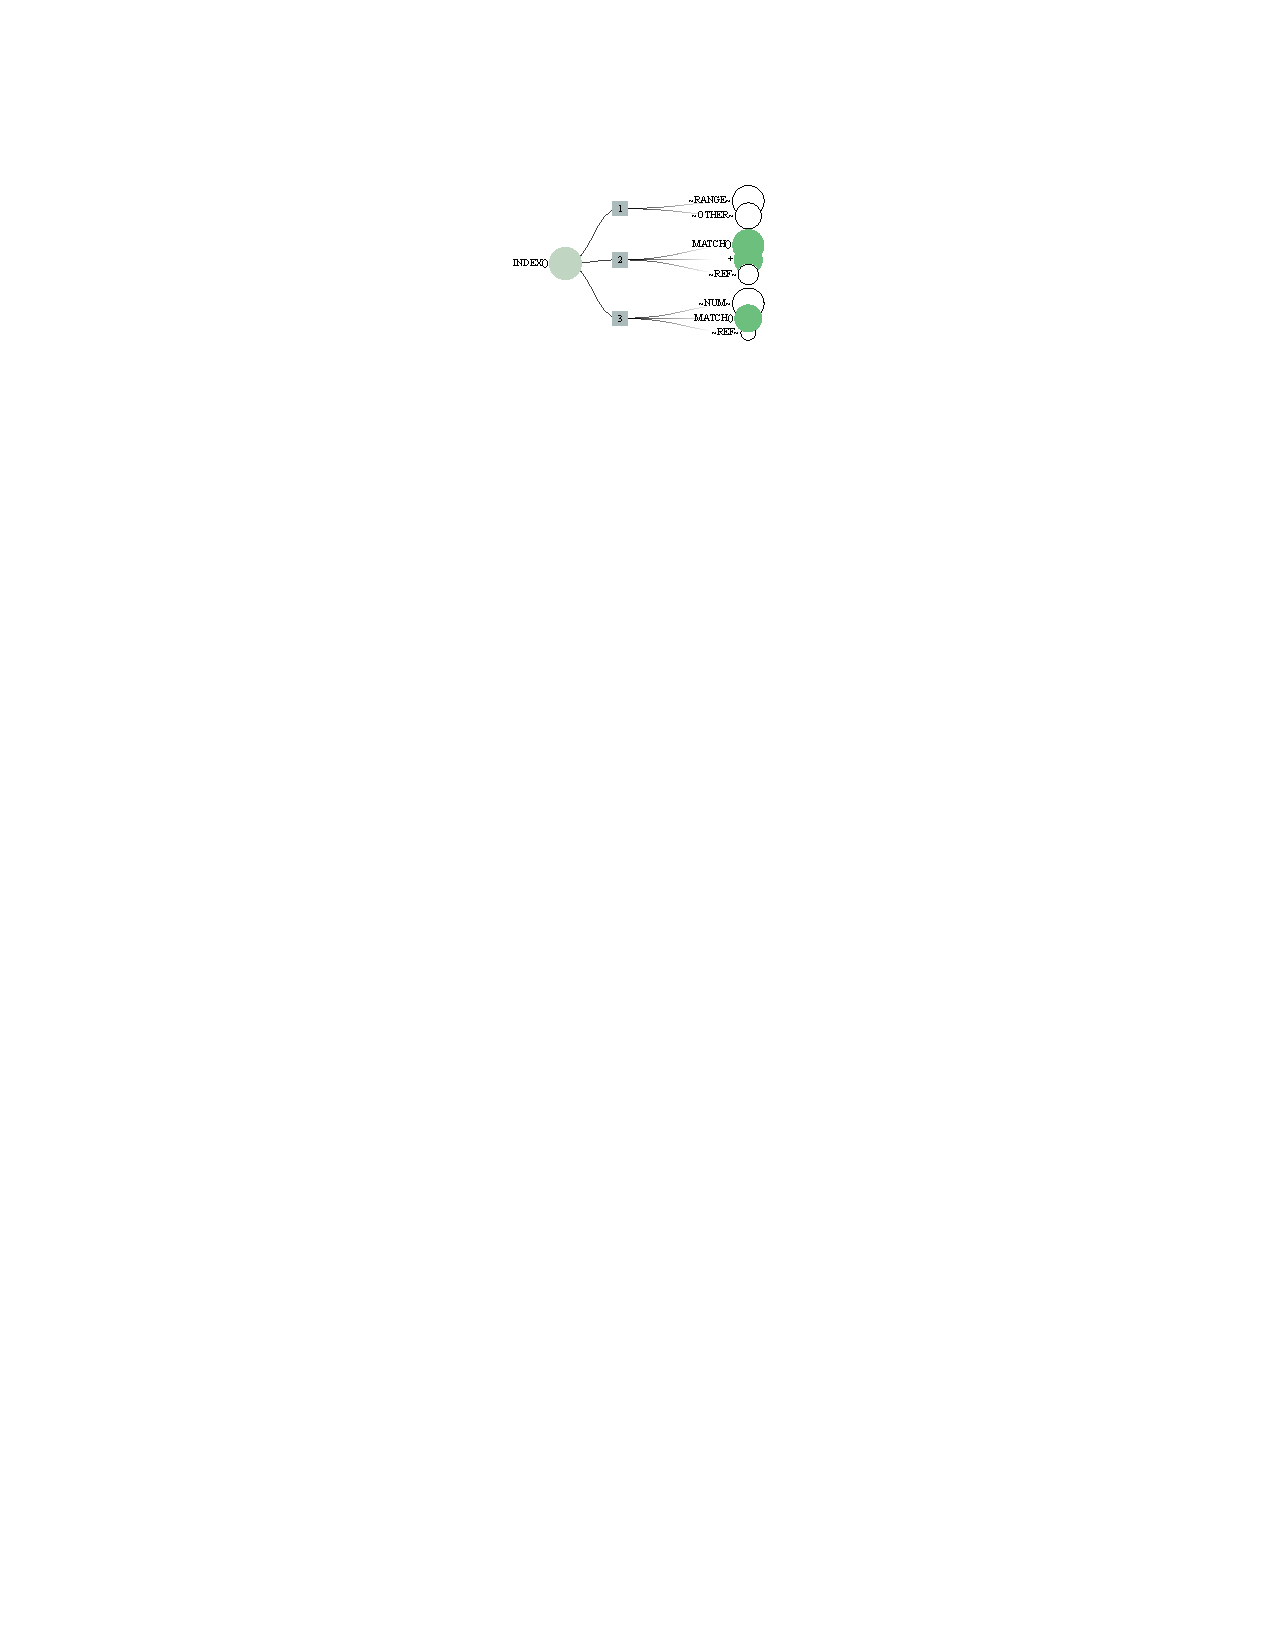
\includegraphics[width=.4\textwidth]{index}
		\caption{A difficult question: how often is MATCH used in both the second and
			third arguments?} \label{fig:index} \end{figure}
	
	Though our focus was specifically on function combination, there are several
	other elements of a formula's context that we do no currently consider. For
	example, \toolname does not current capture argument combination; in Figure
	\ref{fig:index}, it is impossible to state how often the function MATCH
	occurred in both the second and third arguments or whether they were more often
	paired with references. Furthermore, it is easy to open a tree and see what is
	used inside of a specific function, but finding information on what a function
	is used inside of takes considerably more work -- we see again in Figure
	\ref{fig:index} that MATCH is used inside INDEX, but we cannot know which
	functions have INDEX inside them without searching every other tree. More
	distant concerns might be exploring which functions often occur in adjacent
	cells in the sheet -- whenever INDEX occurs, which functions are seen most
	often in the cells around it?
	
	%\begin{wrapfigure}{O}{.25\textwidth} \centering
	%	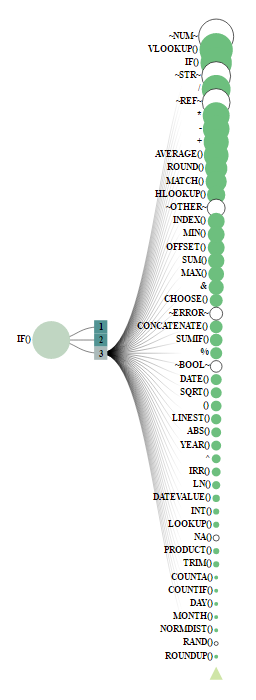
\includegraphics[width=.25\textwidth]{longIF} \label{fig:longif} \caption{The
	%		many possibilities of IF, argument 3, demonstrate the problem of having too
	%		many options.} \end{wrapfigure}
	
	
	
	\section{Conclusion} This paper presents a tool to support the exploration of
	function combinations throughout a given spreadsheet dataset. By taking an
	agnostic approach to design quality, it attempts to convey the dataset's
	spreadsheet practices as is: the common along with the anomalous, and the
	well-designed along with the odorous. As seen in the user and case studies,
	this allows it to take on several potential roles at once, such as an
	environment for investigating code smells as well as a repository for examples
	for learning new techniques. \par
	
	The design of the tool still has much room for improvement. Though the
	exploratory philosophy fostered certain goals well, such as the ability to
	discover new problematic smells without knowing beforehand what they are, it
	hindered others. Some users, for example, found the trees of popular functions
	to be too crowded to explore well, or that their intention to use the tool to
	examine the good or the bad design exclusively was not fully supported by a
	tool that claimed to know neither. Many of the problems, however, were not
	essential to this design conflict and will be overcome in future iterations of
	design by refining icons and improving maneuverability. \par
	
	Either way, the visualization of these large datasets represents an important
	step in improving practice overall. By taking these voluminous oceans of data
	offered in spreadsheet corpora and rendering them comprehensible through
	visualization, we seek to draw attention to valuable information that would
	otherwise go unnoticed.
	
	% use section* for acknowledgment
	\section*{Acknowledgment} This material is based upon work supported in whole
	or in part with funding from the Laboratory for Analytic Sciences (LAS). Any
	opinions, findings, conclusions, or recommendations expressed in this material
	are those of the author(s) and do not necessarily reflect the views of the LAS
	and/or any agency or entity of the United States Government. I also thank the
	anonymous reviewers who advised the direction of this paper.
	
	% references section
	
	% can use a bibliography generated by BibTeX as a .bbl file
	% BibTeX documentation can be easily obtained at:
	% http://mirror.ctan.org/biblio/bibtex/contrib/doc/
	% The IEEEtran BibTeX style support page is at:
	% http://www.michaelshell.org/tex/ieeetran/bibtex/
	\bibliographystyle{IEEEtran} % argument is your BibTeX string definitions and
	% bibliography database(s)
	\bibliography{paper} %
	% <OR> manually copy in the resultant .bbl file
	% set second argument of \begin to the number of references
	% (used to reserve space for the reference number labels box)
	%\begin{thebibliography}{1}
	%
	%\bibitem{IEEEhowto:kopka}
	%H.~Kopka and P.~W. Daly, \emph{A Guide to \LaTeX}, 3rd~ed.\hskip 1em plus
	%  0.5em minus 0.4em\relax Harlow, England: Addison-Wesley, 1999.
	%
	%
	%\end{thebibliography}
	
	
	
	
	% that's all folks
\end{document}

